\documentclass[a4paper,12pt]{article} 

%%% Работа с русским языком
\usepackage{cmap}                           % поиск в PDF
\usepackage{mathtext} 			 	       % русские буквы в формулах
\usepackage[T2A]{fontenc}               % кодировка
\usepackage[utf8]{inputenc}              % кодировка исходного текста
\usepackage[english,russian]{babel}  % локализация и переносы
\usepackage{wrapfig}
\usepackage{gensymb}
\usepackage{textcomp}
\usepackage{multirow}
\usepackage{amsmath,amsfonts,amssymb,amsthm,mathtools} % AMS
\usepackage{euscript}	 % Шрифт Евклид
\usepackage{mathrsfs} % Красивый матшрифт
\usepackage{graphicx}%Вставка картинок правильная
\usepackage{float}%"Плавающие" картинки
\usepackage{wrapfig}%Обтекание фигур (таблиц, картинок и прочего)
\title{Лабораторная работа 1.3.3 

Измерение вязкости воздуха по течению в тонких трубках}
\author{Кагарманов Радмир Б01-106}
\date{6 мая 2022 г.}

\begin{document}

\maketitle
\thispagestyle{empty}
\newpage
\setcounter{page}{1}
\paragraph{Цель работы:}экспериментально исследовать свойства течения газов по тонким трубкам при различных числах Рейнольдса; выявить область применимости закона Пуазейля и с его помощью определить коэффициент вязкости воздуха.
\paragraph{В работе используется:}В работе используются: система подачи воздуха (компрессор, поводящие трубки); газовый счетчик барабанного типа; спиртовой микроманометр с регулируемым наклоном; набор трубок различного диаметра с выходами для подсоединения микроманометра; секундомер.
\paragraph{Теоретические сведения\\}
Работа посвящена изучению течения воздуха по прямой трубе круглого сечения. Движение жидкости или газа вызывается перепадом внешнего давления на концах $\Delta P$ трубы, чему в свою очередь препятствуют силы вязкого (внутреннего) трения, действующие между соседними слоями жидкости, а также со стороны стенок трубы.

Сила вязкого трения как в жидкостях, так и в газах описывается законом
Ньютона: касательное напряжение между слоями пропорционально перепаду
скорости течения в направлении, поперечном к потоку. В частности, если жидкость течёт вдоль оси x,  а скорость течения $v_{x}(y)$ зависит от координаты $y$  в каждом слое возникает направленное по $x$ касательное напряжение.

Величину $\eta$ называют коэффициентом динамической вязкости (или просто вязкостью) среды.

Объёмным расходом (или просто расходом) $Q$ называют объём жидкости,
протекающий через сечение трубы в единицу времени. Величина $Q$ зависит от
перепада давления $\Delta P$, а также от свойств газа (плотности $\rho$ и вязкости $\eta$) и от
геометрических размеров (радиуса трубы $R$ и её длины $L$). Основная задача
данной работы — исследовать эту зависимость экспериментально.

Характер течения в трубе может быть ламинарным либо турбулентным. 

Характер течения определяется безразмерным параметром задачи — числом Рейнольдса
\begin{equation}
    Re = \frac{\rho \bar u a}{\eta},
\end{equation}

где $\rho$ - плотность жидкости, $\bar u = \frac{Q}{\pi R^2} = \frac{U_{max}}{2}$ - средняя скорость движения потока, $a$ - характерный размер потока.\\
Объёмный расход жидкости $Q$ можно найти по формуле:
\begin{equation}
    Q=\frac{\pi R^4 \Delta P}{8\eta l}
\end{equation}
Длина установления $l_{уст}$:
\begin{equation}
    l_{уст}=0,2R \cdot Re
\end{equation}
\paragraph{Экспериментальная установка\\}
Схема экспериментальной установки изображена на Рис. 1. Поток воздуха
под давлением, немного превышающим атмосферное, поступает через газовый счётчик в тонкие металлические трубки. Воздух нагнетается компрессором, интенсивность его подачи регулируется краном К. Трубки снабжены
съёмными заглушками на концах и рядом миллиметровых отверстий, к которым можно подключать микроманометр. В рабочем состоянии открыта заглушка на одной (рабочей) трубке, микроманометр подключён к двум её выводам, а все остальные отверстия плотно закрыты пробками.\\
Перед входом в газовый счётчик установлен водяной U-образный манометр. Он служит для измерения давления газа на входе, а также предохраняет
счётчик от выхода из строя.
\begin{figure}[!h]
\centering
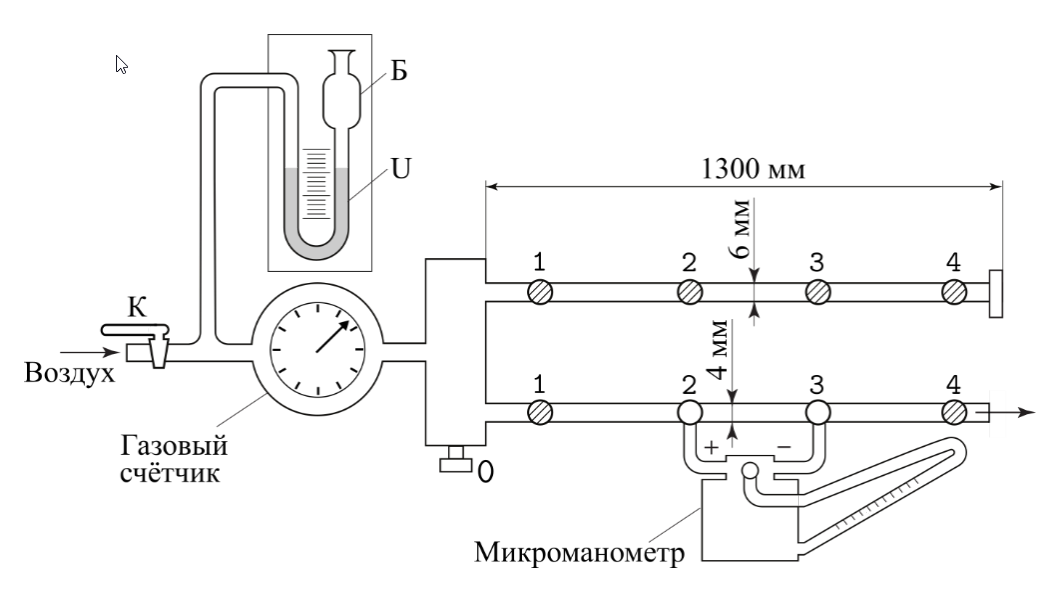
\includegraphics[width=0.8\linewidth]{Экспериментальная установка.png}
\caption{Экспериментальная установка}
\label{fig:mpr}
\end{figure}
\paragraph{Ход работы\\}
\subparagraph{1.} $\Delta P$ будем считать по формуле:
\begin{center}
    $\Delta P= 0,2 * 9,8067 * 0,9932 * n$,
\end{center}
где $n$ - количество делений на микроманометре. Домножаем на 0,9932, так как температура была $24\degree C$.\\
На Рис. 2 и Рис. 3 изображены графики $Q(\Delta P)$ для трубок с диаметрами $d_1=3,90\pm 0,05$ мм и $d_2=5,25\pm 0,05$ мм.
\begin{figure}[!h]
\centering
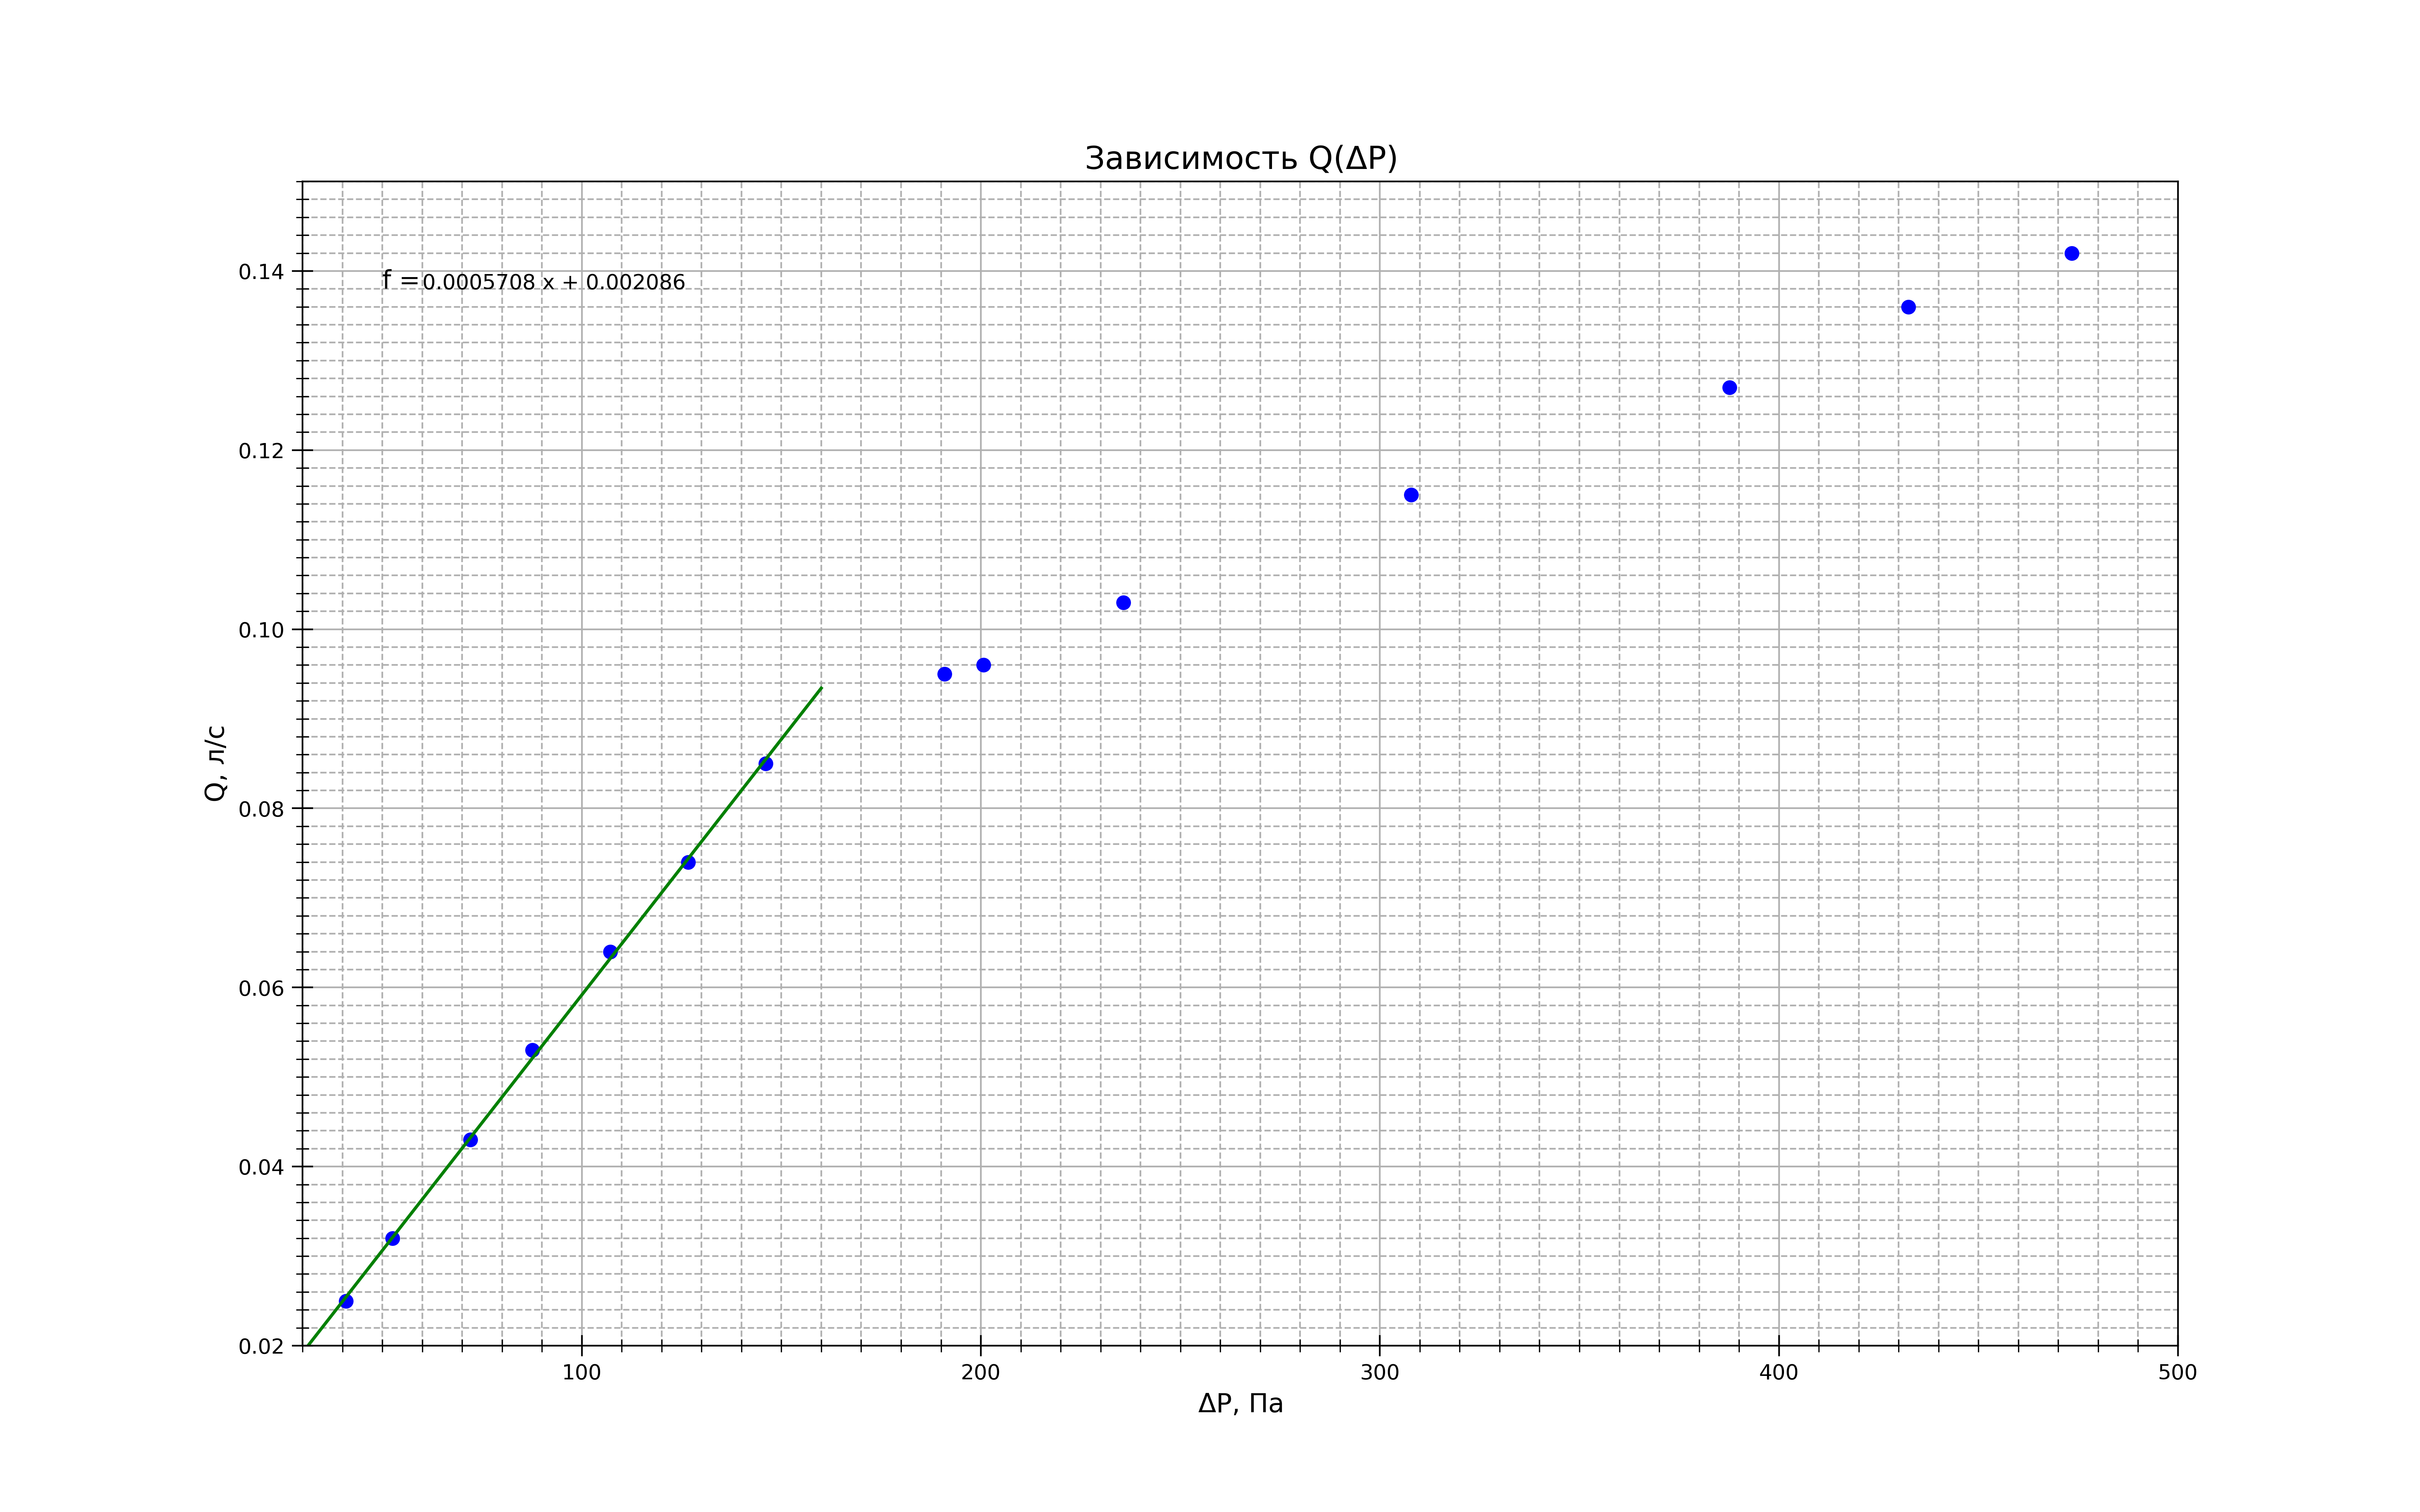
\includegraphics[width=1\linewidth]{QP1.png}
\caption{Зависимость $Q(\Delta P)$ для трубки с диаметром $d_1=3,90\pm 0,05$ мм}
\label{fig:mpr}
\end{figure}
\newpage
\begin{figure}[!h]
\centering
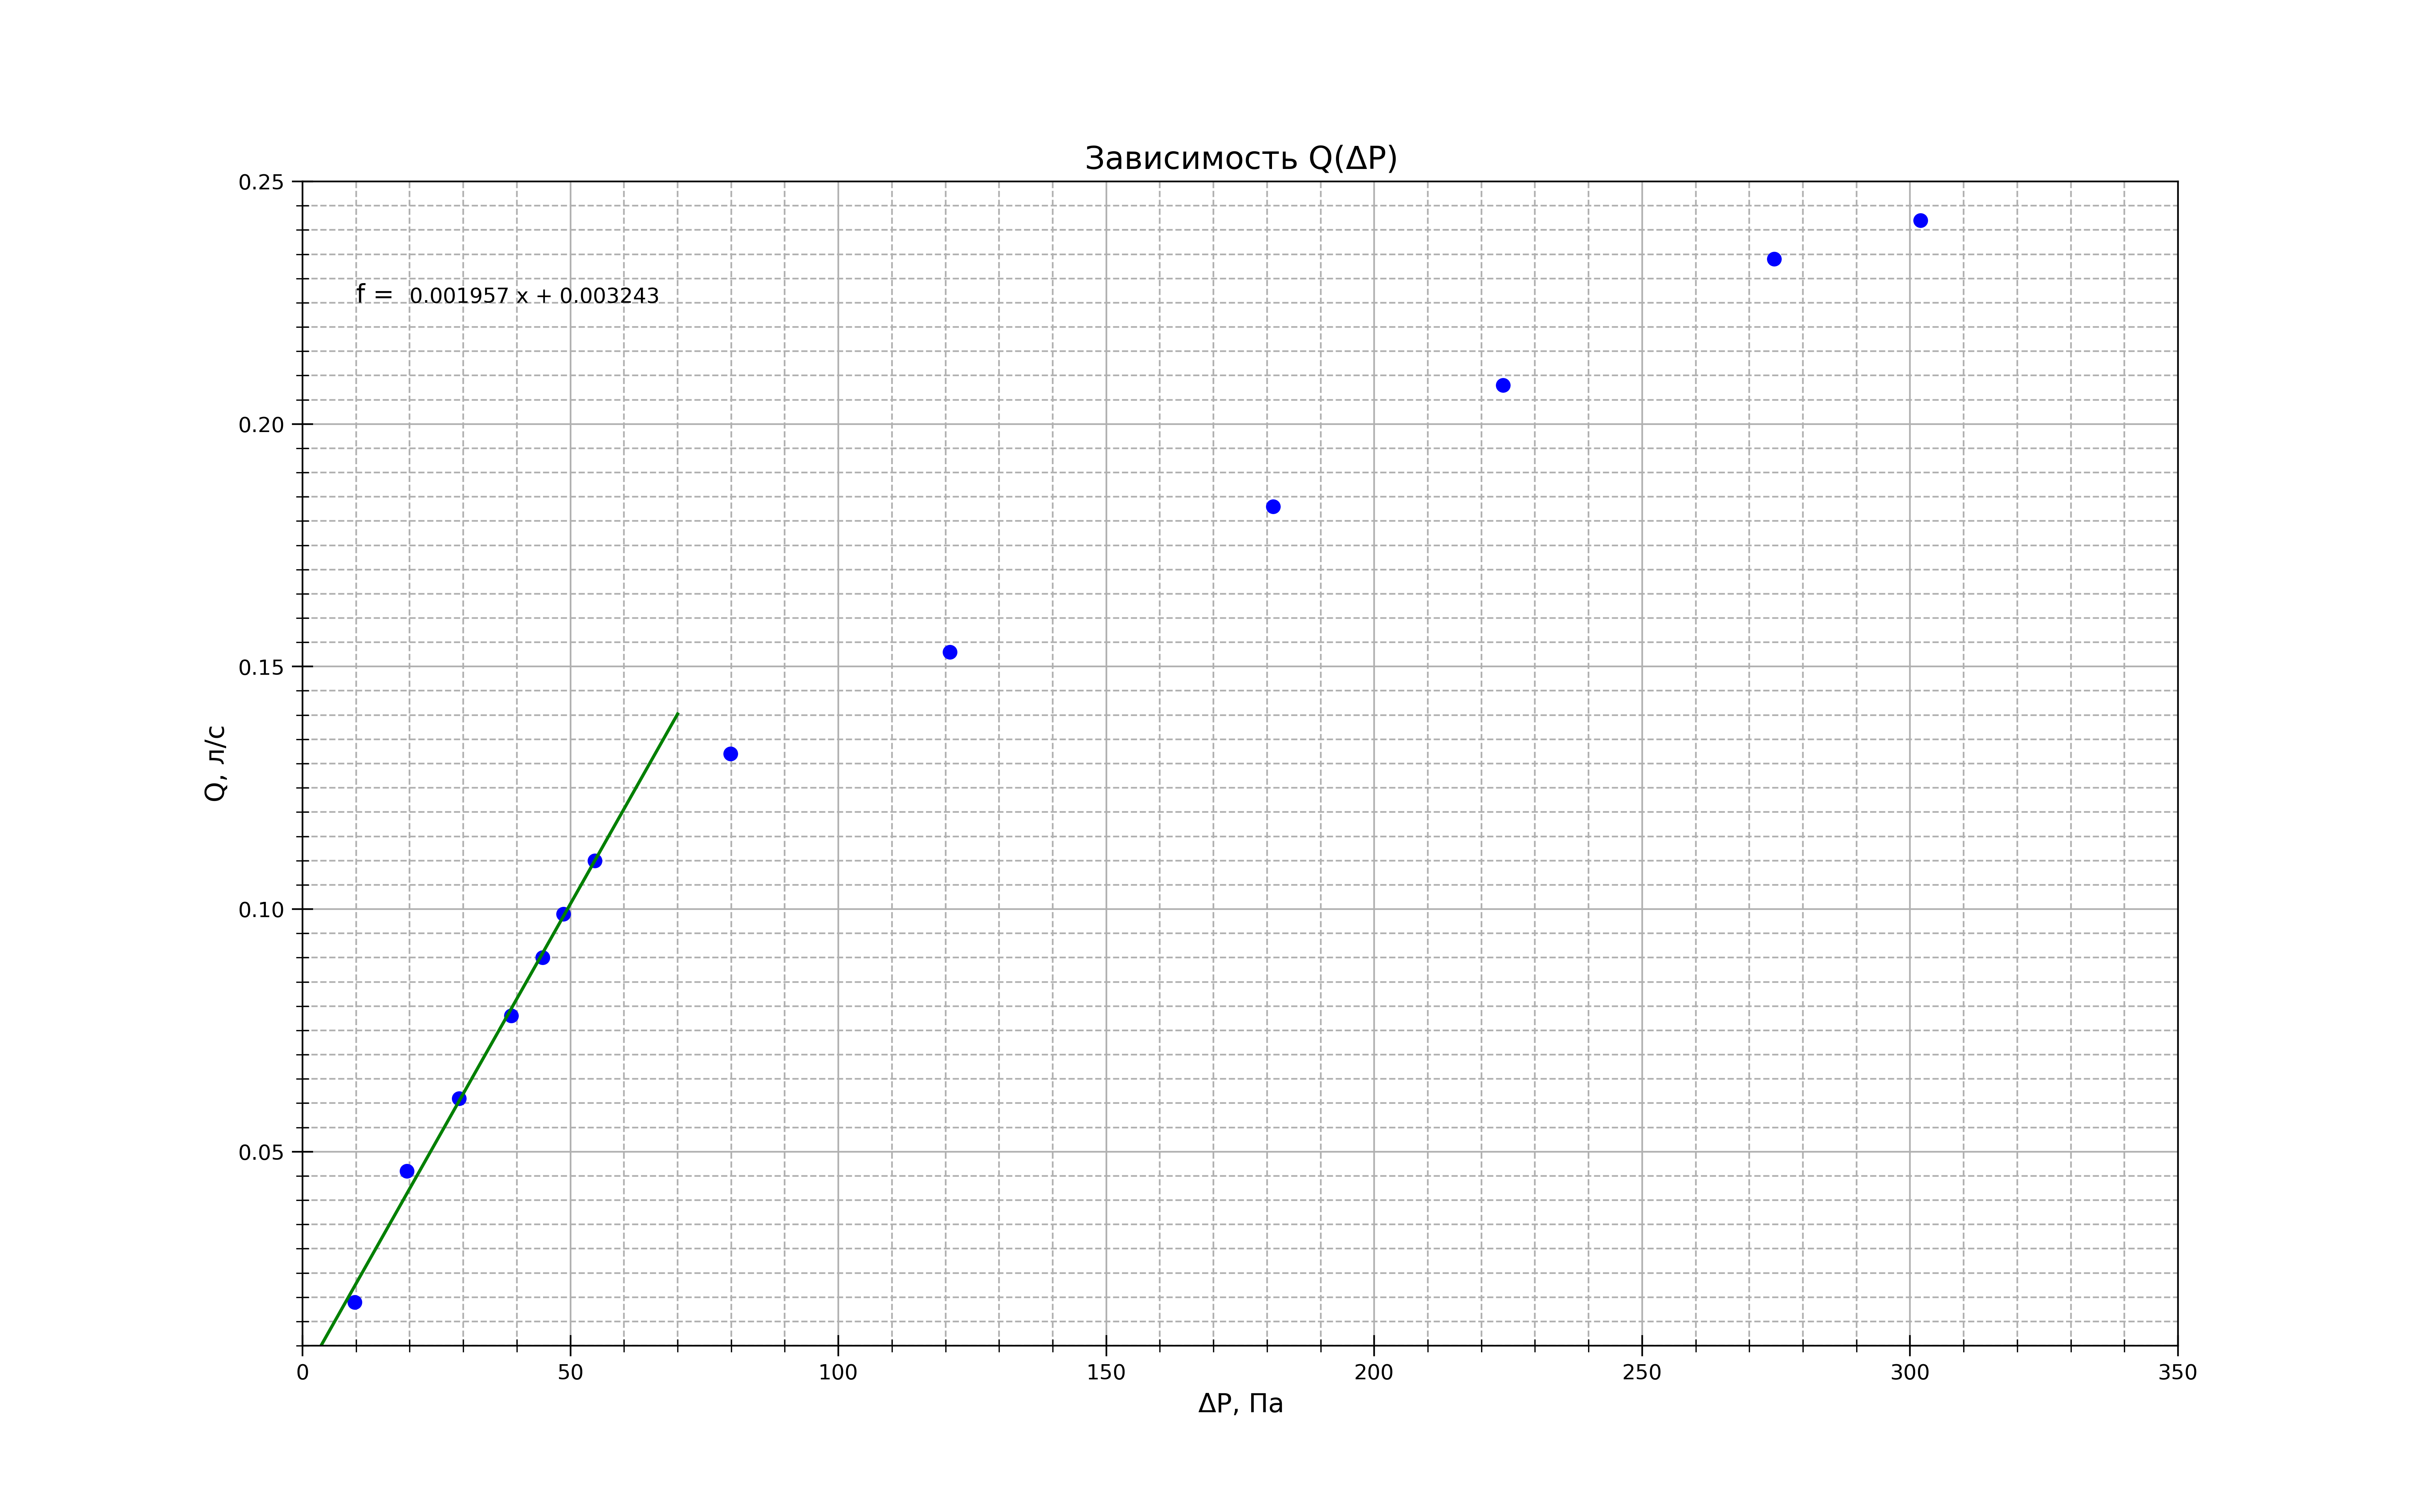
\includegraphics[width=1\linewidth]{QP2.png}
\caption{Зависимость $Q(\Delta P)$ для трубки с диаметром $d_2=5,25\pm 0,05$ мм}
\label{fig:mpr}
\end{figure}
На графиках видно, что для первых 7 измерений зависимость линейная. Из первого графика по формуле (1) $\eta = 1,99\cdot 10^{-5}\pm 0,06\cdot 10^{-5} ~Па \cdot с$. Для второго: $\eta=1,90\cdot 10^{-5}\pm 0,07\cdot 10^{-5}~ Па \cdot с$.\\
Погрешность $\eta$ находится по формуле:
\begin{center}
    $\varepsilon_{\eta}=\sqrt{\varepsilon_{k}^2 + 4\cdot \varepsilon_{R}^2}$,
\end{center}
где относительная погрешность для $\varepsilon_{k_1}=1\%$ и $\varepsilon_{k_2}=2,9\%$.\\
Как мы видим, $\eta$ совпадает в пределах погрешности для разных трубок.
\paragraph{2.} На Рис. 4 и Рис.5 изображены графики зависимости $P(x)$. Посчитав по формуле длины установления получились $l_{уст1}\approx 0,32~ м ~ и ~ l_{уст2}\approx 0,39~ м$. И это видно на графиках.
\begin{figure}[!h]
\centering
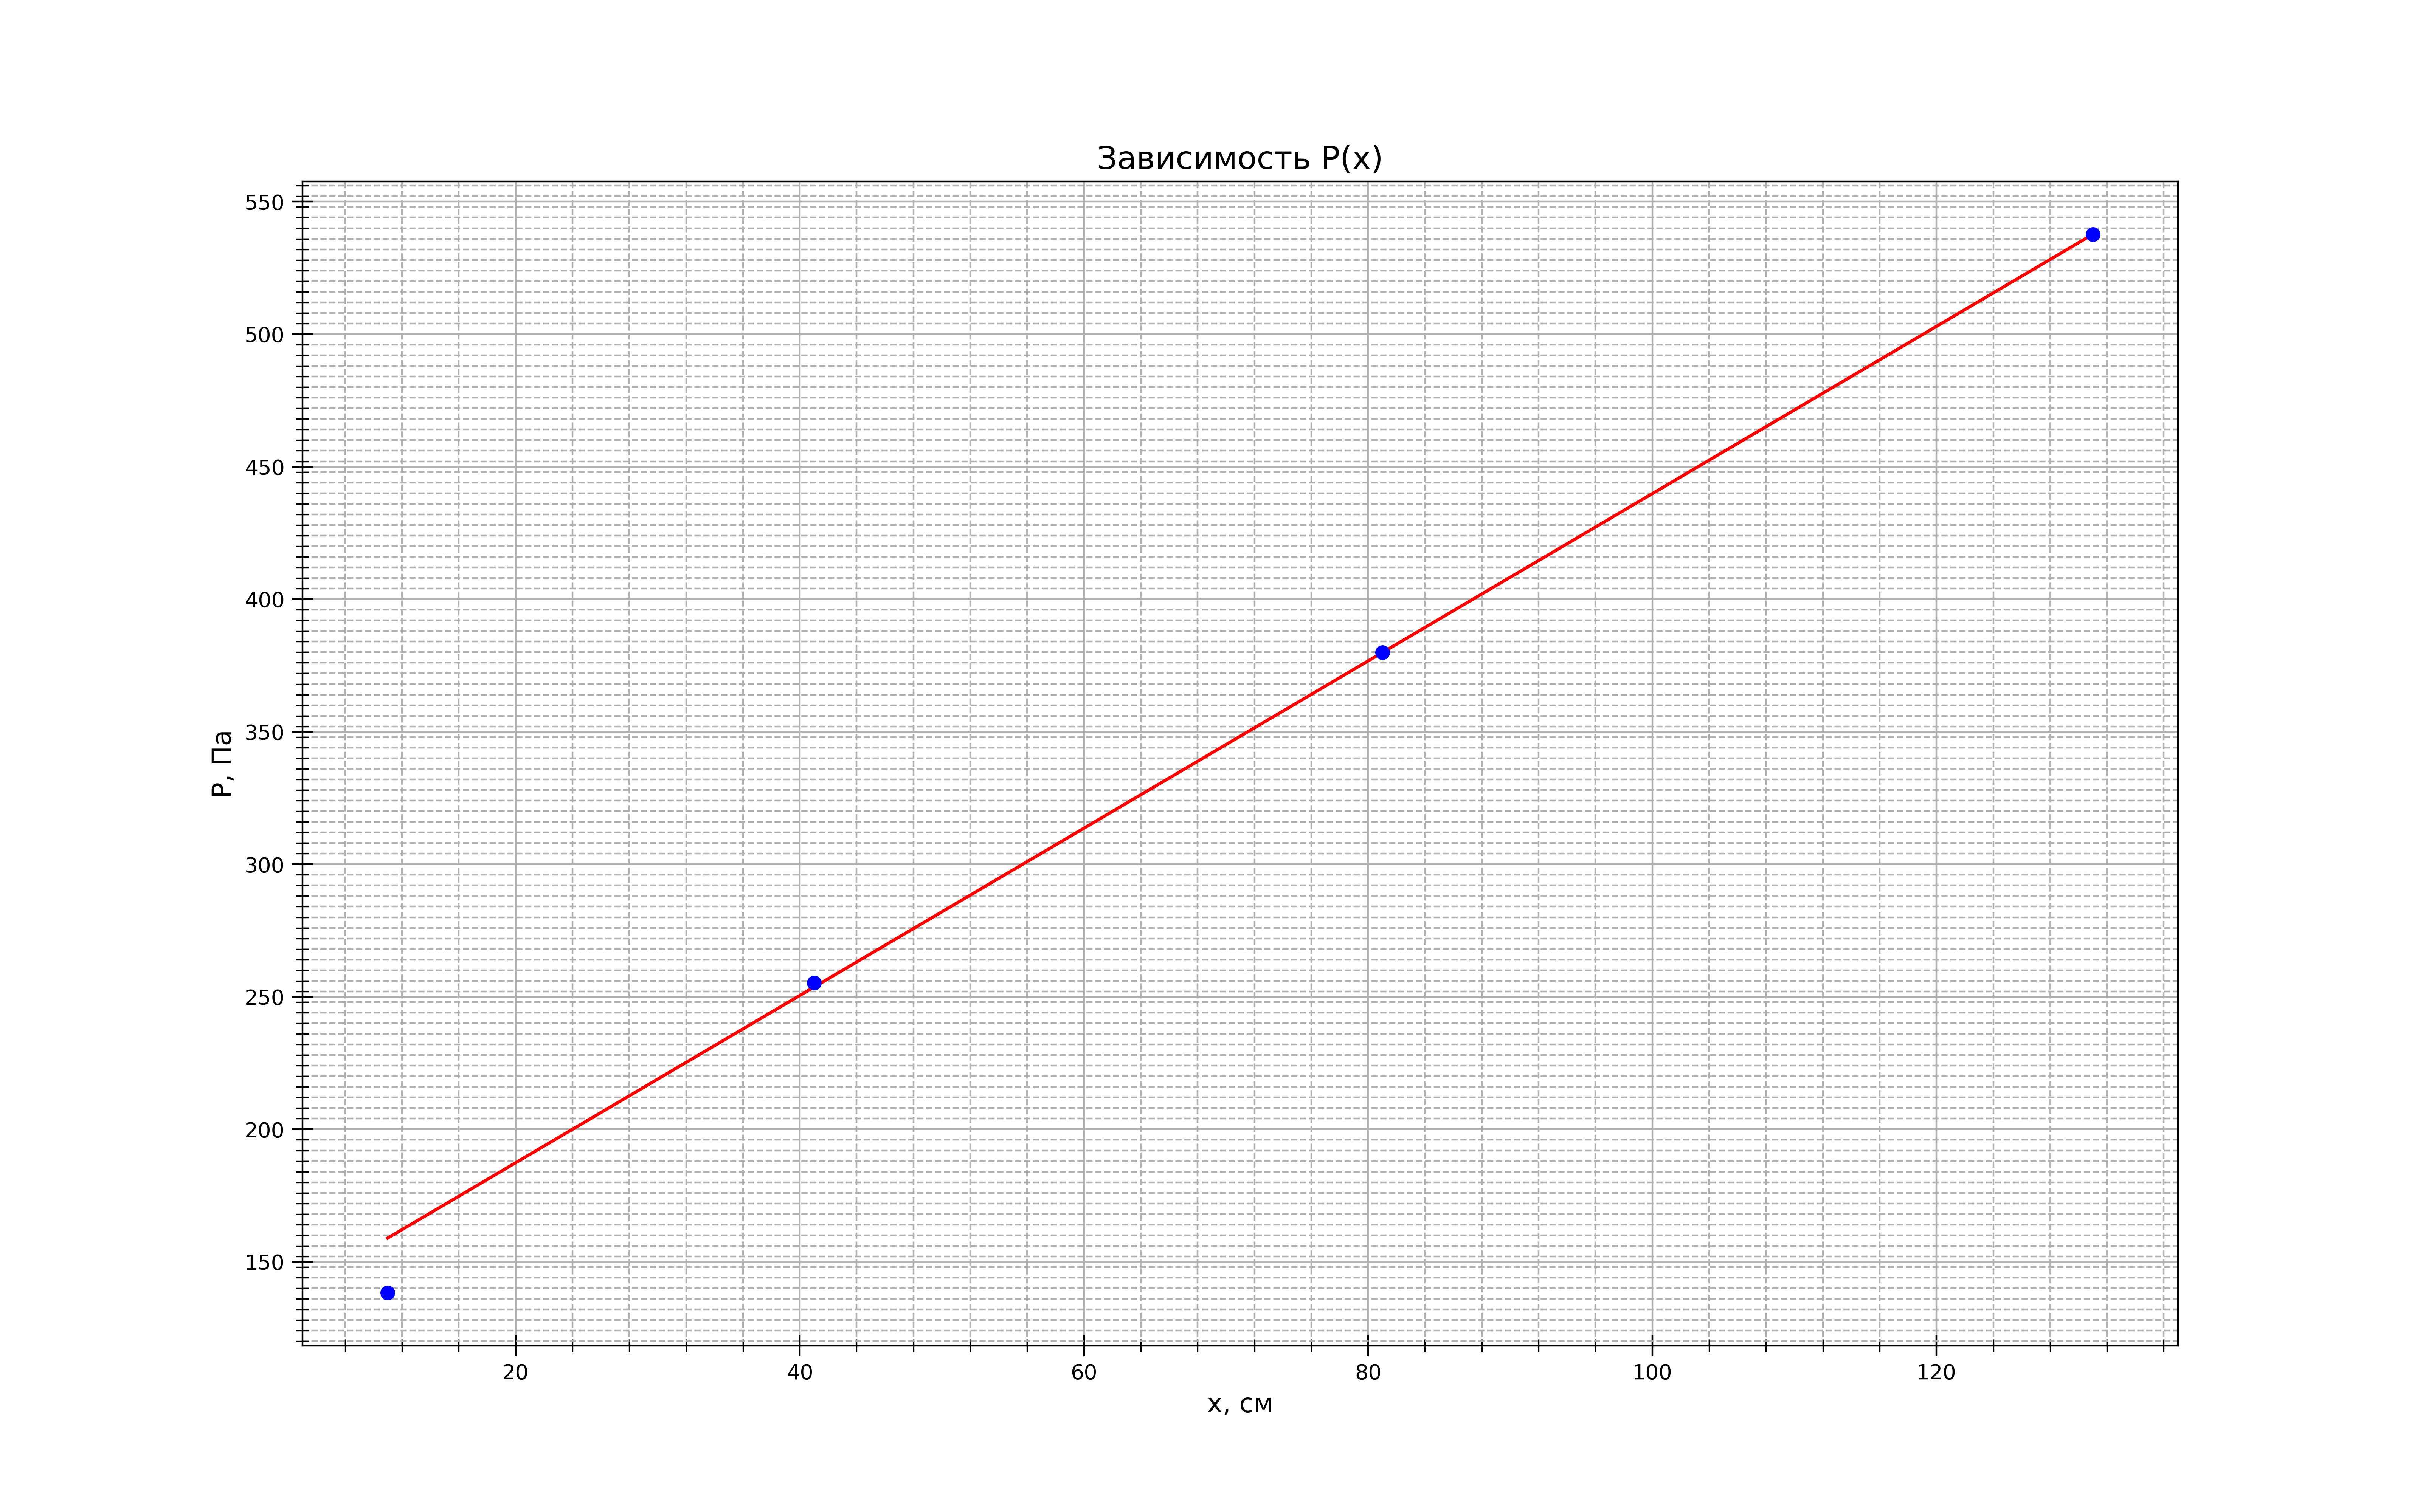
\includegraphics[width=1\linewidth]{P(x)1.png}
\caption{Зависимость $P(x)$ для трубки с диаметром $d_2=5,25\pm 0,05$ мм}
\label{fig:mpr}
\end{figure}
\begin{figure}[!h]
\centering
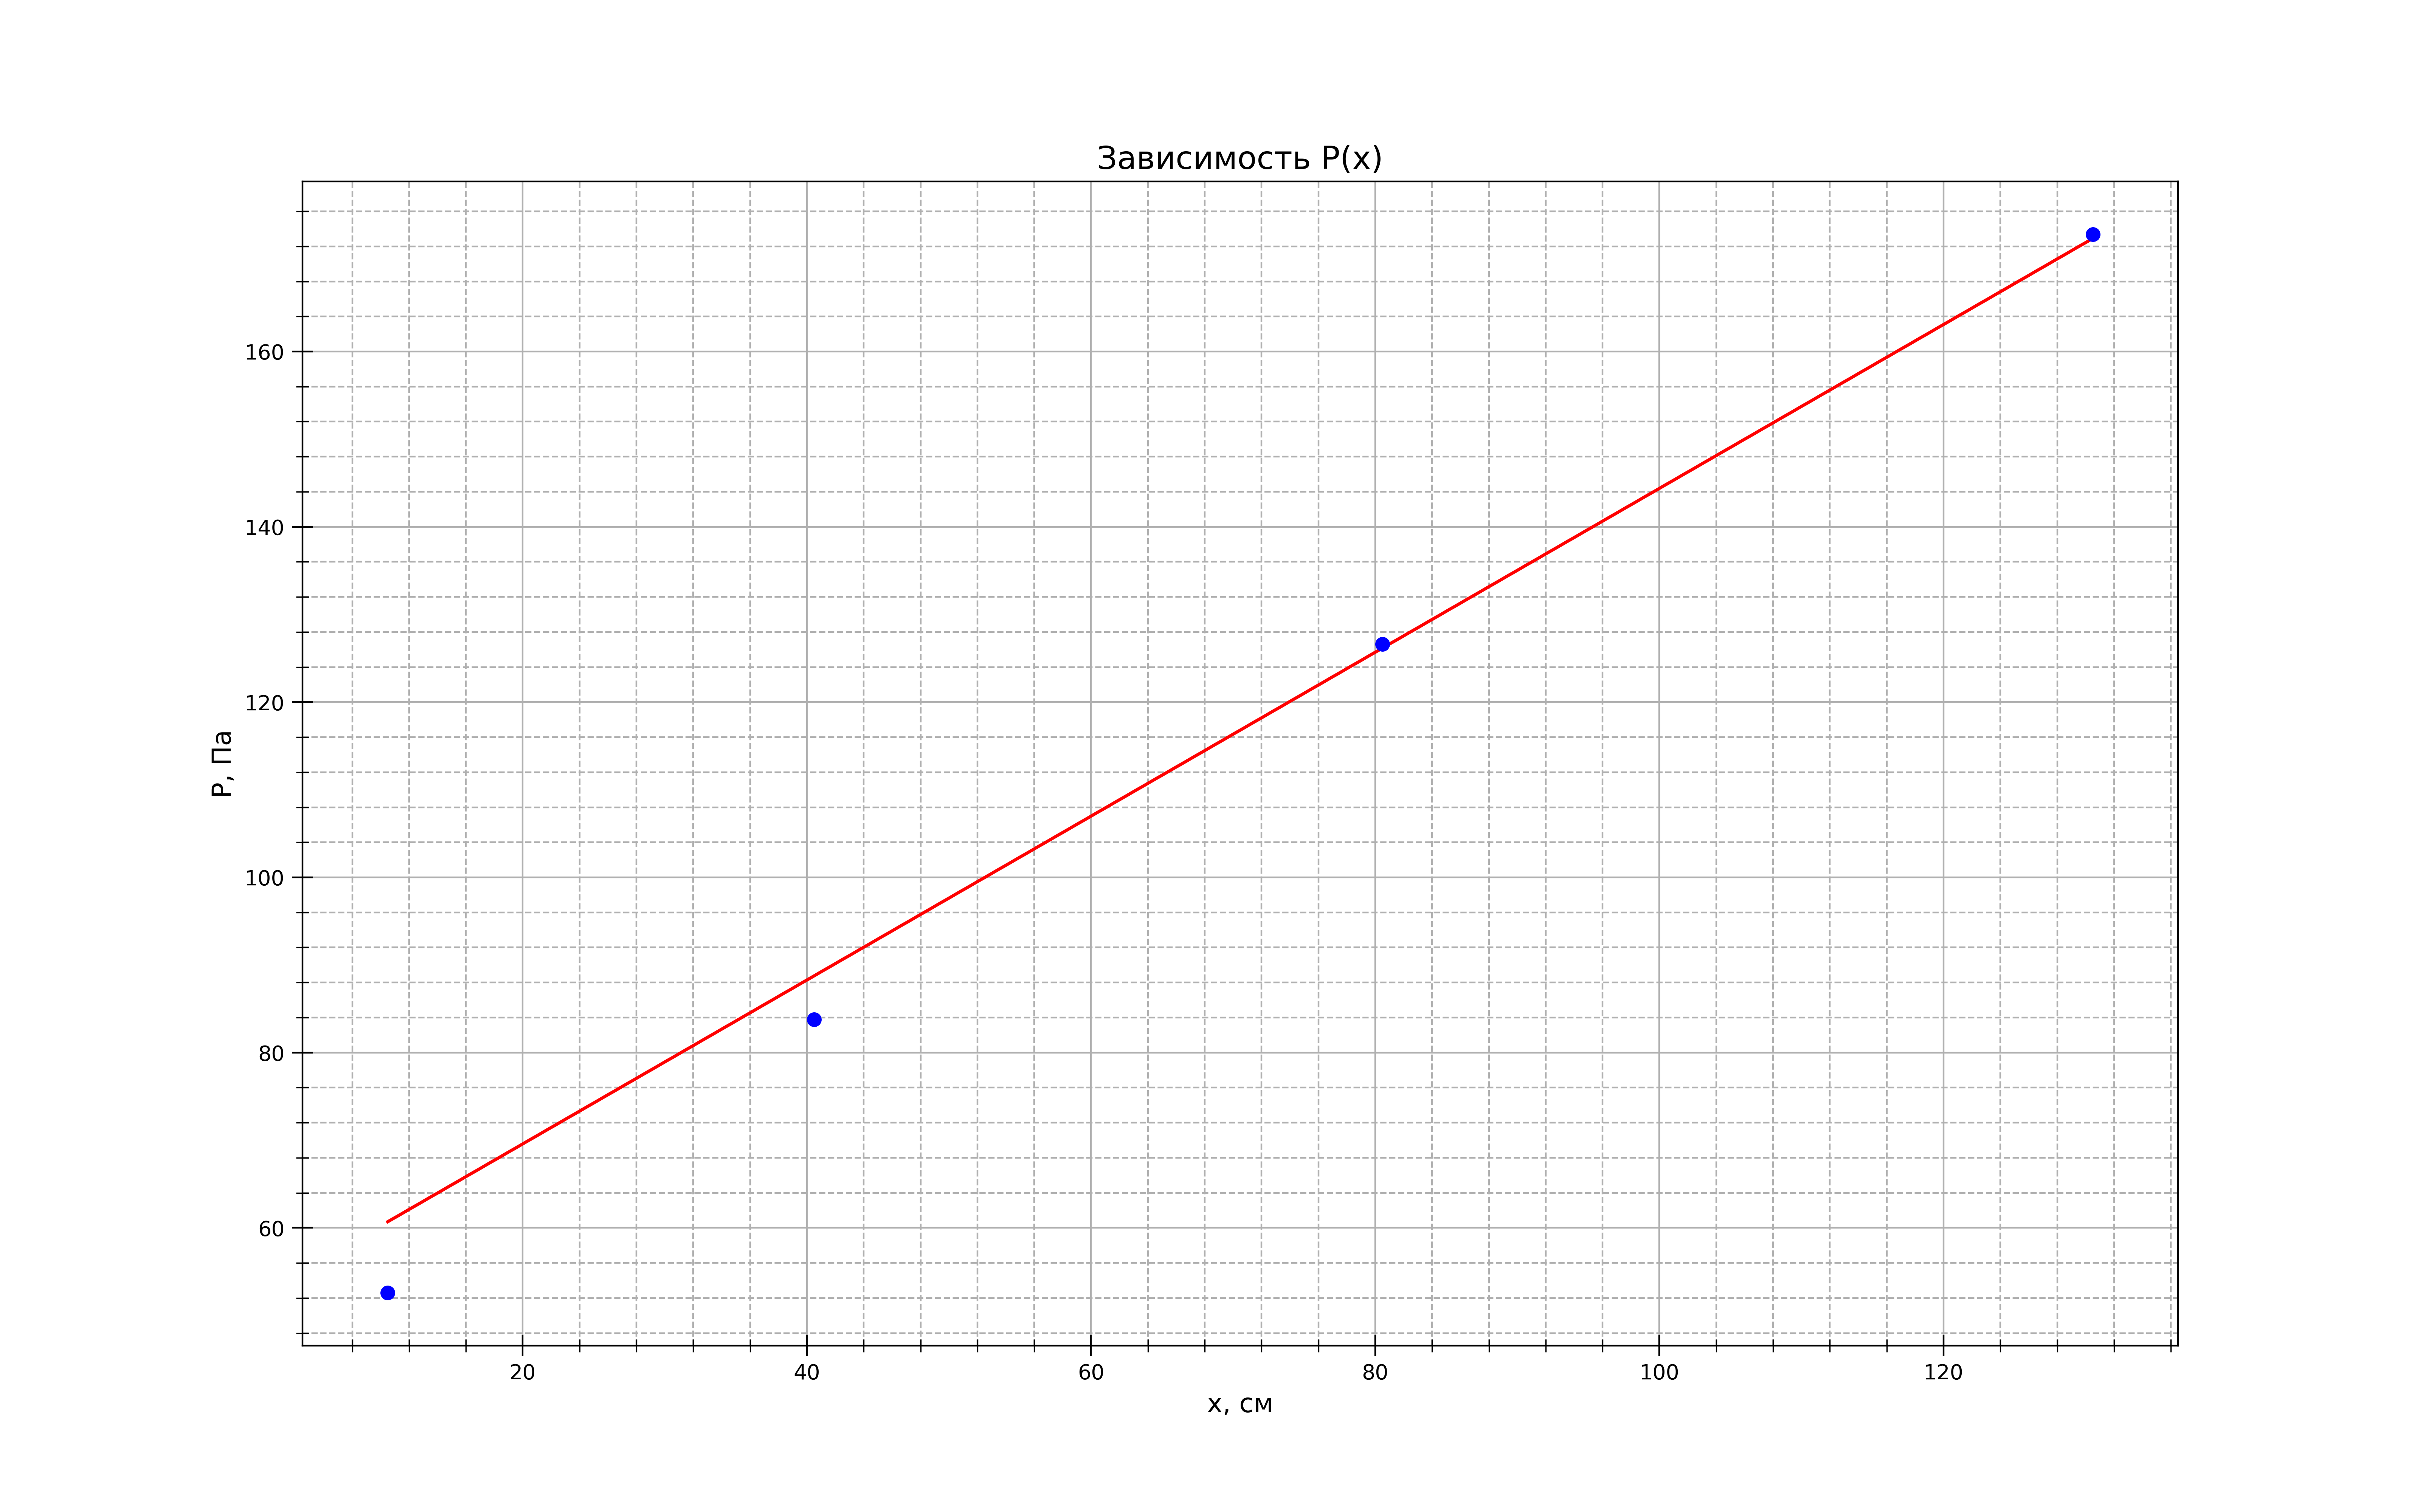
\includegraphics[width=1\linewidth]{P(x)2.png}
\caption{Зависимость $P(x)$ для трубки с диаметром $d_2=5,25\pm 0,05$ мм}
\label{fig:mpr}
\end{figure}
\newpage
\subparagraph{3.}Рассмотрим зависимость $ln Q$ от $ln R$. Она изображена на Рис. 6. С её помощью мы можем найти $\beta$ в $Q\propto R^{\beta}$. Получилось, что $\beta = 4,05\pm 0,13$. Так как расход был в ламинарном режиме, то результат близок к теории.
\begin{figure}[!h]
\centering
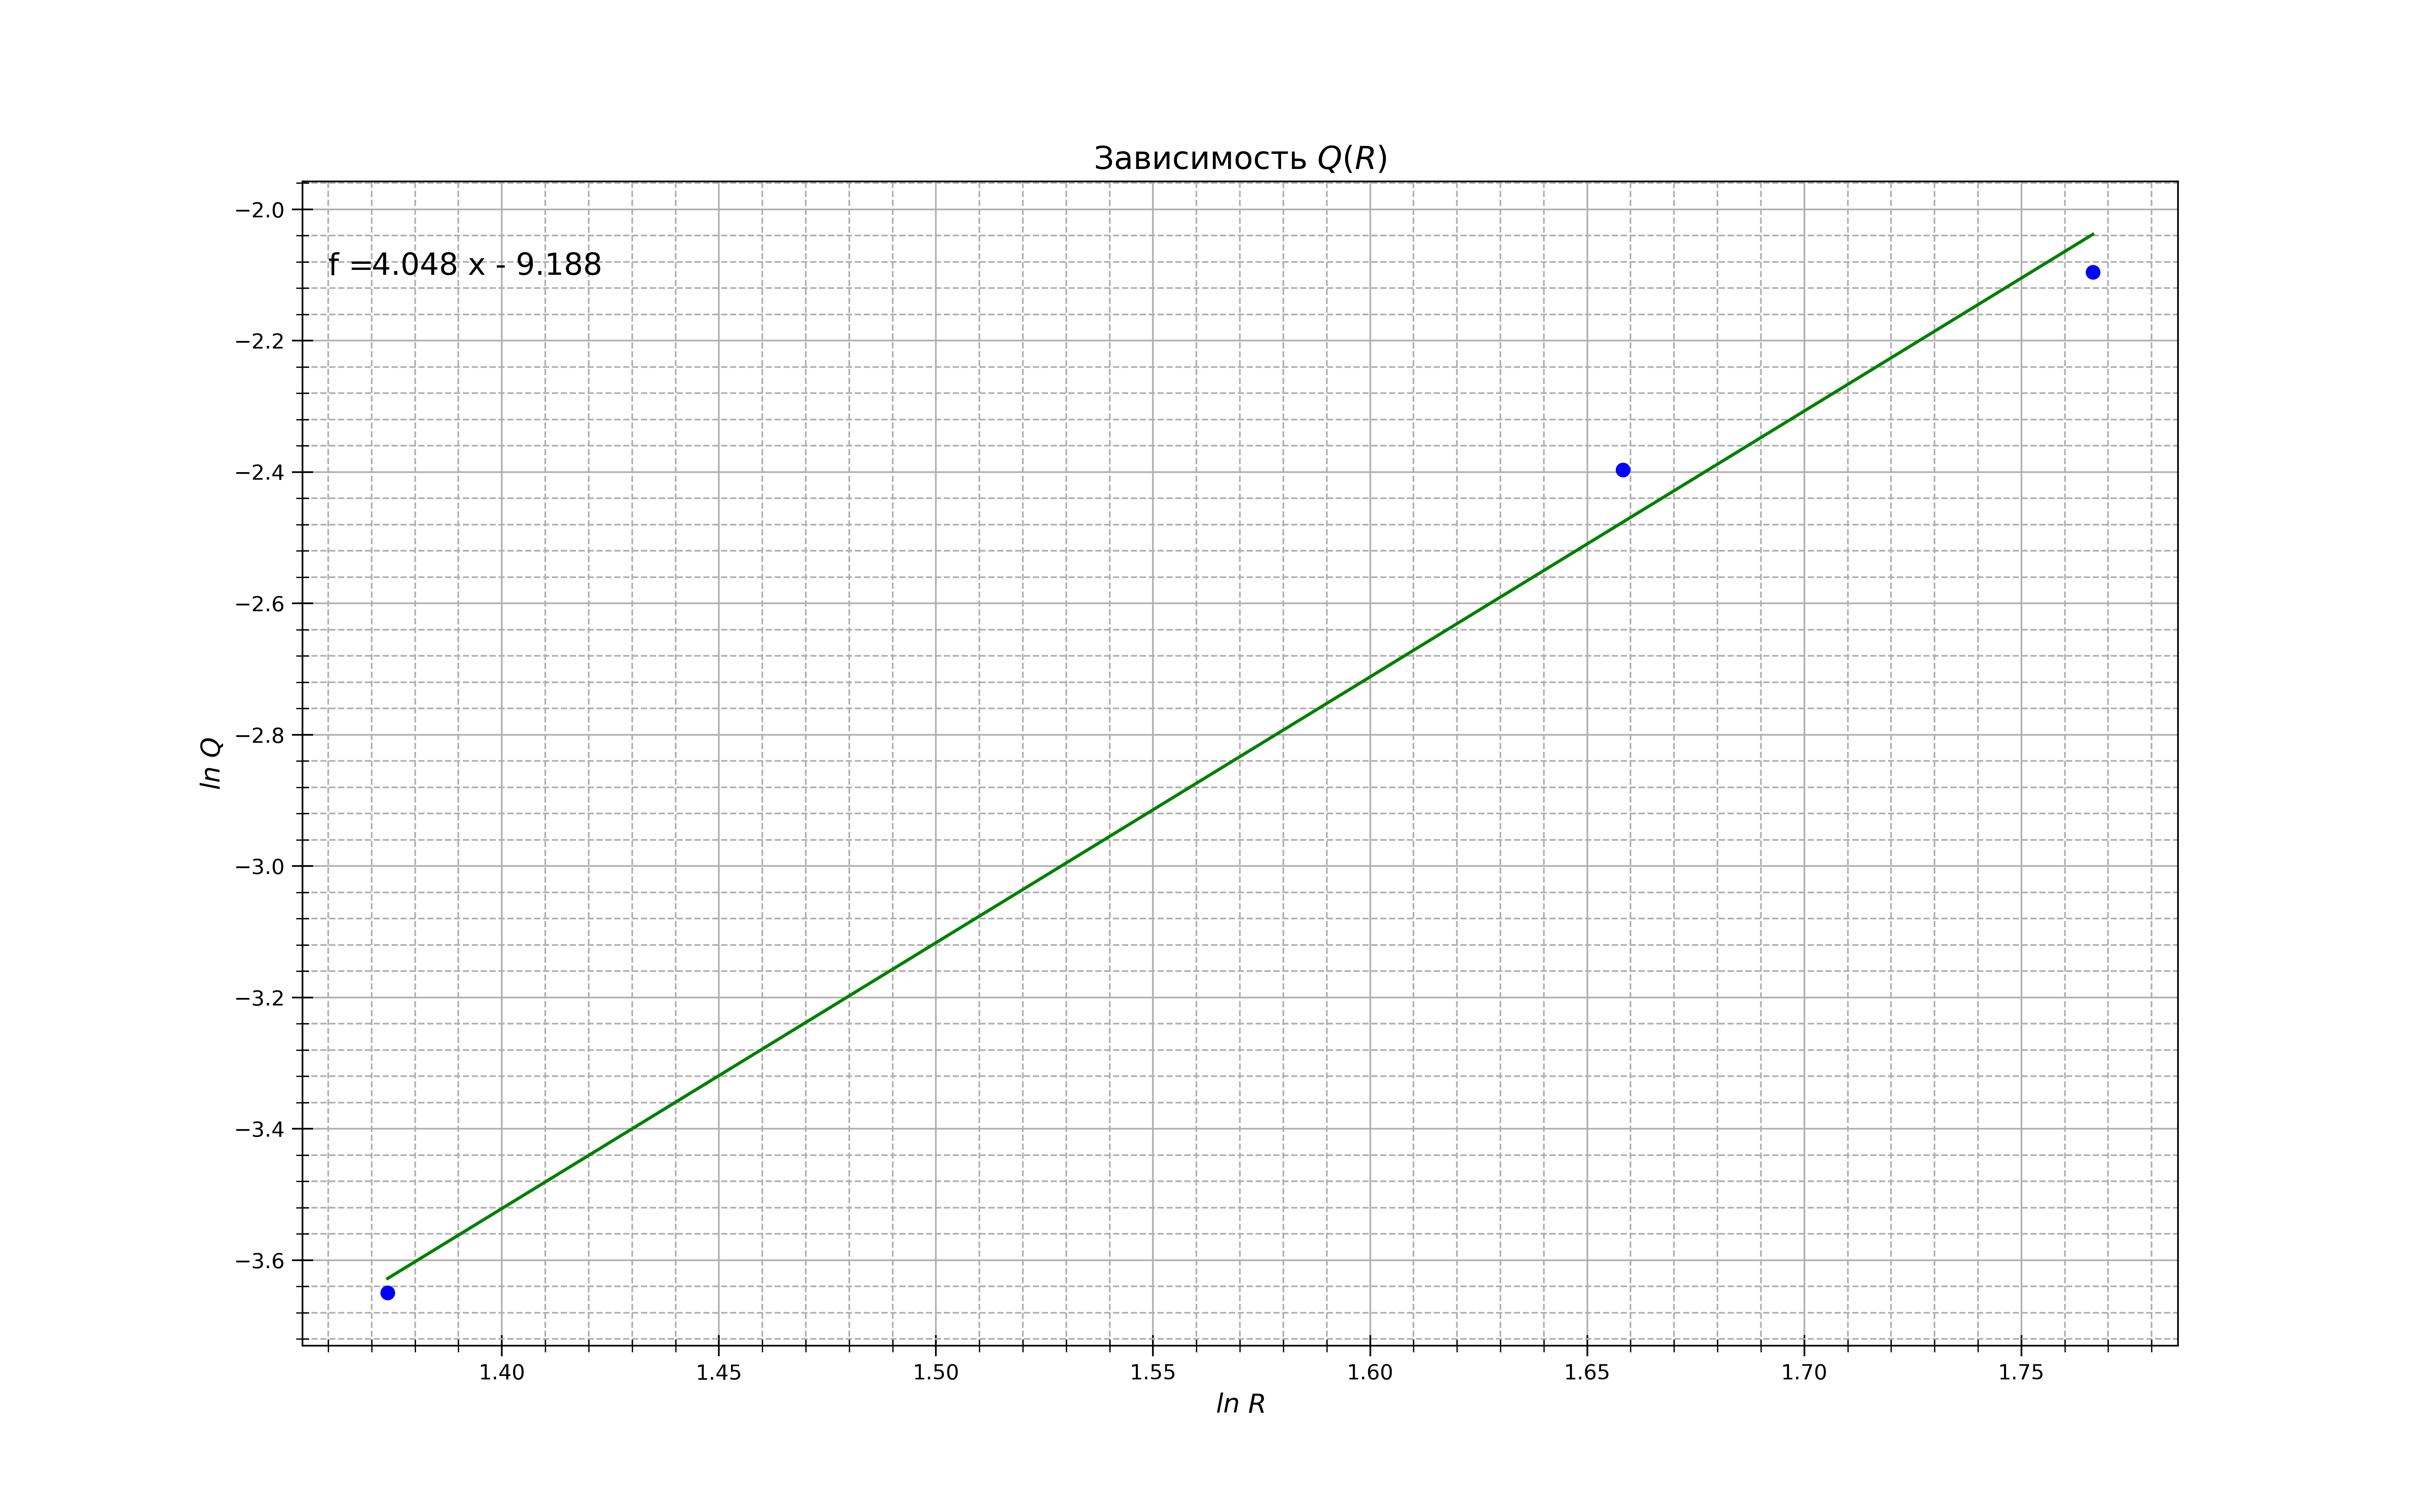
\includegraphics[width=1\linewidth]{Q(r).png}
\caption{Зависимость $ln Q$ от $ln R$}
\label{fig:mpr}
\end{figure}
\paragraph{Вывод:} в данной лабораторной работе мы нашли коэффициент вязкости воздуха $\eta = 1,99\cdot 10^{-5}\pm 0,06\cdot 10^{-5}~ Па\cdot с$ и $\beta = 4,05\pm 0,13$. Также мы рассмотрели зависимость $P(x)$.
\end{document}
